% Certificador: componente de PPA que "certifica" las demostraciones,
%     generando un certificado en deducción natural. Implicó escribir muchos
%     meta-teoremas.
%     \begin{itemize}
%         \item Formalización de muchos teoremas y axiomas: contextos (vale en el prefijo)
%         \item Proof y proof steps, simplificación de la interfaz y mapeo de
%         comandos a steps
%         \item Implementación de cada comando
%         \item By y solver para resolver varios. DNF. Extensión con foralls
%         consecutivos. Demostración / justificación de que es correcto y completo
%         para LP, pero heurístico para LPO (mostrar un caso en el que no funcione)
%         \item Descarga de conjunciones
%         \item Uso de dneg elim como razonamiento por el absurdo para demostrar
%         deMorgan y equivalencias.
%     \end{itemize}

En la sección anterior vimos cómo usar PPA para demostrar teoremas. Pero, ¿cómo
funciona por detrás? ¿Cómo asegura la validez lógica de las demostraciones
escritas por el usuario?

\section{Certificados}

Los programas de PPA se \textbf{certifican}, generando un certificado: una
demostración en deducción natural. ¿Por qué? El lenguaje es complejo, la
implementación no es trivial. Si se programa una demostración, para confiar en
que es correcta hay que confiar también en la implementación de PPA. Pero si
generara una demostración de bajo nivel, que use las reglas de un sistema lógico
simple y conocido, entonces cualquiera que desconfíe podría fácilmente escribir
un chequeador independiente, o usar uno confiable. Decimos que un asistente de
demostración que cuenta con esta propiedad cumple con el
\textbf{criterio de de Bruijn}. \ppaTool{} lo cumple al generar demostraciones
en deducción natural.

\begin{criterion*}[Criterio de de Bruijn \cite{freek-bruijn}] Un asistente de
    demostración que satisface que sus demostraciones puedan ser chequeadas por
    un programa independiente, pequeño y confiable se dice que cumple con el
    criterio de de Bruijn.
\end{criterion*}

%\duda{Para pablo: pero si emite certificados que no corresponden a la demo original y chequean siempre, por ej. siempre el mismo, no estaría mal igual? Tenés que confiar también en la parte que emite el certificado.}
% RTA: Sí, o tendrías que poder mirar qué es lo que se está demostrando. Ese es un problema insalvable.

El módulo de PPA que certifica las demostraciones de alto nivel de PPA
generando una demostración en deducción natural es el \modCertifier{}. Si
bien toda demostración que genere debería ser correcta, para atajar posibles
errores siempre se chequean con el \modChecker{}, el pequeño módulo que implementa el chequeo de los certificados.

\section{Contextos}

Durante el proceso de certificación, en realidad no se genera una sola
demostración, sino que al poder haber más de un teorema en
un programa de PPA, el certificado es un \textbf{contexto} compuesto por una
lista ordenada de \textbf{hipótesis} de dos tipos:

\begin{itemize}
    \item \textbf{Teoremas}: son fórmulas con demostraciones de deducción natural
    asociadas.
    \item \textbf{Axiomas}: son fórmulas que se asumen válidas (pueden ser usadas para
    modelar una teoría)
\end{itemize}

\begin{figure}[h]
    \centering
    \begin{multicols}{2}
        \begin{tabular}{c}
            \lstinputlisting{listings/certifier/two-theorems.ppa}
        \end{tabular}
        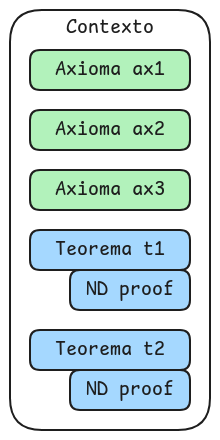
\includegraphics[scale=0.5]{img/ppa-context.png}
    \end{multicols}
    \caption{Contexto resultante de certificar de un programa}
    \label{ppa-cert:fig:context}
\end{figure}


Se puede ver un ejemplo en la \namedref{ppa-cert:fig:context}. También se puede ver
en el tipo de la función principal del módulo: \mintinline{haskell}{certify ::
Program -> Result Context}. Como para un programa generamos muchas
demostraciones, debemos extender el chequeo a contextos: Cada demostración será
válida en el \textit{prefijo estricto del contexto} que la contiene. Es decir, a
la hora de chequear la demostración de un teorema, se deben asumir como ciertas
todas las hipótesis que fueron definidas antes que él. En el ejemplo, cuando
chequeamos la demostración de \lstinline{t1}, debemos asumir como válidos los
axiomas \lstinline{ax1, ax2, ax3}.

\subsection{Contexto local}

No solo los axiomas y teoremas declarados en el programa se agregan al
contexto. Cada demostración de un teorema tendrá además un \textit{contexto
local} que extiende al anterior, solo válido durante el alcance de su
demostración (se omiten en el certificado).

En él, las afirmaciones auxiliares que no afectan la tesis como
\lstinline{have}, \lstinline{claim} y \lstinline{consider}, etc. se agregan como
teoremas. Por lo tanto, cuando se citen, se pueden copiar sus demostraciones tomándolas del contexto local. Por otro
lado, algunos comandos agregan axiomas, los mismos que en deducción natural
agregan fórmulas al contexto (\lstinline{suppose} y \lstinline{consider}). Es
correcto asumir como ciertas esas hipótesis, porque lo mismo se hará durante el
chequeo de la demostración generada de deducción natural. Se puede ver un
ejemplo en la \fullref{ppa-cert:fig:local-context}.

\begin{figure}[h]
    \centering
    \begin{multicols}{2}
        \begin{tabular}{c}
            \lstinputlisting{listings/certifier/local-context.ppa}
        \end{tabular}
        \vfill\null
        \columnbreak
        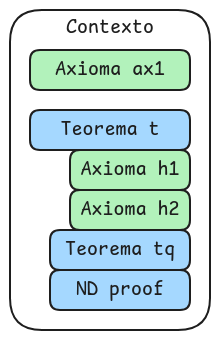
\includegraphics[scale=0.5]{img/ppa-local-context.png}
    \end{multicols}
    \caption{Contexto local}
    \label{ppa-cert:fig:local-context}
\end{figure}

\section{Certificado de demostraciones}

Ya vimos cómo las hipótesis se agregan al contexto. Pero ¿cómo generamos una demostración de deducción natural a partir de una demostración de un teorema de \ppaLang{}? Para cada comando introducido en el \namedref{chap:ppa}, deberemos \textit{certificarlo} generando una demostración, y el resto del programa debería demostrar sus premisas. En la \namedref{ppa-cert:certify:ex} se puede ver un ejemplo, en donde \lstinline{take} se certifica como \ruleExistsI{}, y la demostración de su premisa está dada por el certificado del resto del programa, \lstinline{thus p(v) by ax}, que se certifica como \ruleAx.

\begin{figure}[H]
    \begin{multicols}{2}
        \begin{tabular}{c}
            \lstinputlisting{listings/extract/exists.ppa}
        \end{tabular}
        \begin{prooftree}
            \AxiomC{}
            \RL{\ruleAx}
            \UnaryInfC{$p(v) \judG p(v)$}
            \RL{\ruleExistsI}
            \UnaryInfC{$p(v) \judG \exists x . p(X)$}
        \end{prooftree}
    \end{multicols}
    \caption{Ejemplo de certificado generado para un programa}
    \label{ppa-cert:certify:ex}
\end{figure}

En el resto del capítulo presentamos cómo cada comando de \ppaLang{} puede ser certificado.

\begin{itemize} 
    \item Comenzamos por ver cómo se certifican los comandos que corresponden a reglas de inferencia de forma directa, que ayuda a entender el funcionamiento de \ppaTool{}: \lstinline{take} (\ruleExistsI), \lstinline{consider} (\ruleExistsE), \lstinline{let} (\ruleForallI), \lstinline{cases} (\ruleOrE) y \lstinline{suppose} (\ruleImpI, \ruleNotI). También los comandos adicionales: \lstinline{equivalently} y \lstinline{claim}.
    \item Luego, describimos el \textit{solver} que se usa por debajo del \lstinline{by}, que es central al funcionamiento de todo el certificador. Aquí veremos que la demostración generada para \ref{ppa-cert:certify:ex} no es exactamente como se presenta.
    \item Concluimos por cómo podemos usarlo para facilitar la descarga de conjunciones en un orden arbitrario.
\end{itemize}

\section{Comandos correspondientes a reglas de inferencia}

Como se puede ver en \fullref{ppa:tab:inference-rules-to-commands}, muchos de los comandos se corresponden directamente con reglas de inferencia,
por lo que su traducción es directa.

\begin{itemize}
    \item \lstinline{take} (\ruleExistsI)

    Si la tesis es \lstinline{exists X . a}, el comando \lstinline{take X := t}
    la reduce a \lstinline{a} con \lstinline{X} reemplazado por \lstinline{t} y la certifica como
    
    \proofTreeExistsI

    insertando la demostración certificada del resto en en $\ctx \judG \form \subst{\var}{\term}$

    \item \lstinline{consider} (\ruleExistsE)
    
    El comando \lstinline{consider X st h: a by h1, ... hn} se certifica como
    
    \proofTreeExistsE

    \begin{itemize}
        \item $\ctx \judG \exists \var . \form$ se demuestra mediante el by.
        \item Se agrega la hipótesis \lstinline{h: a} al contexto como axioma, se continúa la certificación y se inserta la demostración resultante en $\ctx, \form \judG \formTwo$.
    \end{itemize}

    \item \lstinline{let} (\ruleForallI)
    
    Si la tesis es \lstinline{forall X. a}, el comando \lstinline{let X} reduce la tesis a \lstinline{a} y continúa la certificación, insertando el resultado en la demostración de $\ctx \judG \form$

    \proofTreeForallI

    \item \lstinline{cases} (\ruleOrE)
    
    El comando
    \begin{lstlisting}[numbers=none]
        cases by h1, ..., hn
            case c1
            ...
            case cm
        end
    \end{lstlisting}

    se certifica como varios \ruleOrE{} anidados, en donde el primer $\fOr$ se certifica mediante by. Cada rama certifica la sub-demostración agregando la hipótesis del caso al contexto como axioma.

    \proofTreeOrE

    \item \lstinline{suppose} (\ruleImpI, \ruleNotI)
    
    Si la tesis es \lstinline{a -> b}, el comando \lstinline{suppose h: a} reduce la tesis a \lstinline{b} y agrega al contexto la hipótesis \lstinline{h: a} como axioma. La certifica como

    \proofTreeImpI

    insertando el resto de la demostración certificada en su sub-demostración.

    Si la tesis es \lstinline{~a}, es análogo pero interpretándolo como \lstinline{a -> false}.

\end{itemize}

\section{Comandos adicionales}

\begin{itemize}
    \item \lstinline{equivalently}
    
    Si la tesis es $a$, el comando \lstinline{equivalently a'} usa el mismo solver que el by para demostrar $a' \fImp a$ y reduce la tesis a $a'$.

    \item \lstinline{claim}
    
    La certificación del comando
    \begin{lstlisting}[numbers=none]
claim h: f
proof
    ...
end
    \end{lstlisting}
    
    Consiste en certificar la sub-demostración y agregar la hipótesis \lstinline{h: f} como teorema al contexto.

\end{itemize}


\section{Implementación del by}

El \lstinline{by} es el mecanismo principal de demostración en PPA, y el corazón
del \modCertifier. Muchas funcionalidades están implementadas a su alrededor.
Genera \textbf{automáticamente} una demostración de que una fórmula es
consecuencia lógica de una lista de hipótesis. Es un \textit{solver heurístico} para lógica de primer orden. Esto es aceptable, puesto que la validez de lógica de primer orden es indecidible (por el teorema de Church \cite{church}), y el objetivo del trabajo no fue dar un solver innovador, sino alguno que se pueda certificar. Está basado en la implementación del mecanismo análogo en el \texttt{Checker} de Mizar \cite{freek-by}.

Sea $A$ una fórmula. Supongamos que queremos certificar \lstinline{thus A by h1, ..., hn} y que en el contexto tenemos que las hipótesis $h_i$ corresponden a
fórmulas $\formTwo_i$, con $i \in \{1, ..., n\}$ y $n \in \setNaturals$. Primero
vemos la idea general de la estrategia y luego profundizamos en cada paso. Los pasos para certificar un \lstinline{by} son los siguientes. 
\begin{itemize}
    \item Queremos demostrar la implicación de las hipótesis a la fórmula.
    \[
        \formTwo_1 \fAnd \dots \fAnd \formTwo_n \fImp \form
    \]
    A esta fórmula la llamamos \textbf{tesis}.
    \item \textbf{Razonamos por el absurdo}: asumiendo la negación de la tesis buscamos encontrar una contradicción
    \begin{align*}
        \fNot (\formTwo_1 \fAnd \dots \fAnd \formTwo_n \fImp \form)
        &\equiv \fNot (\fNot (\formTwo_1 \fAnd \dots \fAnd \formTwo_n) \fOr \form)\\
        &\equiv \formTwo_1 \fAnd \dots \fAnd \formTwo_n \fAnd \fNot \form
    \end{align*}
    \item Convertimos la negación de la tesis a forma normal disyuntiva (\textbf{DNF}), una disyunción de cláusulas, cada una de las cuales es una conjunción de literales (fórmulas atómicas afirmadas o negadas, y fórmulas iniciadas por cuantificadores).
    \[
        (\formLit^1_{1} \fAnd \dots \fAnd \formLit^1_{n_1})
        \fOr \dots \fOr
        (\formLit^m_{1} \fAnd \dots \fAnd \formLit^m_{n_m})
    \]

    donde $m \in \setNaturals$ es el número de cláusulas, $n_1, \dots, n_m \in
    \setNaturals$ es la cantidad de fórmulas de cada cláusula y $\formLit^i_j$
    es la $j$-ésima fórmula de la $i$-ésima cláusula.

    \item Buscamos una \textbf{contradicción} refutando cada cláusula individualmente.
    Una cláusula $\formLit_1 \fAnd \dots \fAnd \formLit_n$ será refutable si
    cumple una de las siguientes condiciones.
    \begin{itemize}
        \item Contiene $\fFalse$
        \item Contiene dos fórmulas opuestas ($\formLit, \fNot \formLit$)
        \item Eliminando universales consecutivos y re-convirtiendo a DNF, se
        consigue una refutación ($\fNot \pred(k), \forall \var .\ \pred(x)$)
    \end{itemize}
\end{itemize}

La complejidad del mecanismo no reside solo en tener que realizar todos estos
pasos, sino que el desafío principal fue \textbf{generar la demostración en
deducción natural}. Veamos un ejemplo sin generar la demostración, y sin
eliminar universales.

\begin{ejemplo}[Ejemplo sin cuantificadores]
    Tenemos el siguiente programa

    \begin{figure}[H]
        \centering
        \begin{tabular}{c}
            \lstinputlisting{listings/certifier/by-modus-ponens.ppa}
        \end{tabular}
    \end{figure}

    Para certificar \lstinline{thus b by ax1, ax2} hay que generar una
    demostración para la implicación $\big((a \fImp b) \wedge a \big)\fImp b$.

    \begin{enumerate}
        \item Negamos la fórmula 
        \[ \fNot [ \big( (a \to b) \fAnd a \big) \to b ] \]

        \item La convertimos a DNF
        \begin{align*}
            &\fNot [ \big( (a \to b) \fAnd a \big) \to b ] \\
            &\equiv \fNot [ \fNot \big( (a \to b) \fAnd a \big) \fOr b ]
                && (\form \to \formTwo \equiv \fNot \form \fOr \formTwo)\\
            &\equiv \fNot \fNot \big( (a \to b) \fAnd a \big) \fAnd \fNot b
                && (\fNot(\form \fOr \formTwo) \equiv \fNot \form \fAnd \fNot \formTwo)\\
            &\equiv \big( (a \to b) \fAnd a \big) \fAnd \fNot b
                && (\fNot\fNot \form \equiv \form)\\
            &\equiv (\fNot a \fOr b) \fAnd a \fAnd \fNot b
                 && (\form \to \formTwo \equiv \fNot \form \fOr \formTwo)\\
            &\equiv (\fNot a \fOr b) \fAnd a \fAnd \fNot b
                && ((\form \fOr \formTwo) \fAnd \formThree \equiv (\form \fAnd \formThree) \fOr (\formTwo \fAnd \formThree))\\
            &\equiv
                (\fNot a \fAnd a \fAnd \fNot b)
                \vee
                (b \fAnd a \fAnd \fNot b)
        \end{align*}

        \item Buscamos una contradicción refutando cada cláusula
        \begin{itemize}
            \item En $(\fNot a \fAnd a \fAnd \fNot b)$ tenemos $\fNot a$ y $a$.
            \item En $(b \fAnd a \fAnd \fNot b)$ tenemos $b$ y $\fNot b$.
        \end{itemize}
    \end{enumerate}
\end{ejemplo}

\subsection{Certificado del by}

En el resto de la sección, entramos en detalle de cómo generar una demostración para cada paso del by.

\begin{enumerate}
    \item \fullref{ppa-cert:sec:abs-reasoning}: primero necesitamos una forma de razonar por el absurdo, que nos permita deducir la fórmula original asumiendo su negación y demostrando $\fFalse$. Esto lo hacemos mediante dos reglas admisibles: la eliminación de doble negación (\ruleDnegE{}), equivalente a \ruleLEM{}, y \ruleCut{} que nos permite juntar demostraciones.
    \item \fullref{ppa-cert:sec:dnf}: luego vemos cómo demostrar de forma automática que una fórmula es equivalente a su versión en DNF, que se realiza a partir de un sistema de reescritura.
    \item \fullref{ppa-cert:sec:contradictions}: una vez que la fórmula está en DNF, tenemos que demostrar a partir de ella una contradicción. 
    \item \fullref{ppa:sec:by:forall-elim}: si no se encuentra una contradicción de forma simple, se procede a eliminar $\forall$ consecutivos y reiniciar el proceso pero con unificación de fórmulas en lugar de igualdad, para así instanciar las variables cuantificadas universalmente.
    \item \fullref{ppa-cert:sec:expressiveness}: finalmente evaluamos el alcance y limitaciones del \textit{solver} implementado, que resulta completo para proposicional y heurístico para primer orden.
\end{enumerate}


\subsection{Razonamiento por el absurdo}
\label{ppa-cert:sec:abs-reasoning}

Queremos asumir que no vale la fórmula original, es decir $\fNot (\formTwo_1
\fAnd \dots \fAnd \formTwo_n \fImp \form)$, y llegar a una contradicción. Pero
en la demostración que estamos generando, tenemos que demostrar $(\formTwo_1
\fAnd \dots \fAnd \formTwo_n \fImp \form)$. ¿Cómo se puede razonar por el
absurdo?

De la misma forma que en la \namedref{nd:sec:admissible-rules} se introduce
\textit{modus tollens} como una regla admisible, para razonar por el absurdo
vamos a usar la \textbf{eliminación de la doble negación}. Es un principio de
razonamiento clásico que es equivalente a LEM.


\begin{theorem}[Eliminación de la doble negación]
    Sea $\form$ una fórmula cualquiera. Vale $\fNot \fNot \form \judG \form$, y lo notamos como regla admisible

    \begin{prooftree}
        \AxiomC{}
        \RL{\ruleDnegE}
        \admissibleRuleLine
        \UnaryInfC{$\fNot \fNot \form \judG \form$}
    \end{prooftree}
\end{theorem}
\begin{proof}
    En deducción natural,

    \begin{prooftree}
        \def\defaultHypSeparation{\hskip .1in} % default .2in
        \AxiomC{}
        \LL{\ruleLEM}
        \UnaryInfC{$\fNot \fNot \form \judG \form \fOr \fNot \form$}
        \AxiomC{}
        \RL{\ruleAx}
        \UnaryInfC{\(
            \fNot \fNot \form, \form \judG \form
        \)}
        \AxiomC{}
        \LL{\ruleAx}
        \UnaryInfC{\(
            \fNot \fNot \form, \fNot\form \judG \fNot \fNot \form
        \)}
        \AxiomC{}
        \RL{\ruleAx}
        \UnaryInfC{\(
            \fNot \fNot \form, \fNot\form \judG \fNot \form
        \)}
        \RL{\ruleNotE}
        \BinaryInfC{\(
            \fNot \fNot \form, \fNot \form \judG \form
        \)}
        \RL{\ruleOrE}
        \TrinaryInfC{$\fNot \fNot \form \judG \form$}
    \end{prooftree}
\end{proof}

¿Cómo lo usamos? Introducimos otra regla admisible: \textbf{cut}, que nos
permite ``pegar'' demostraciones entre sí. Si estamos queriendo demostrar
$\form$, y queremos reducir el problema a $\formTwo$ que sí podemos probar, esta
regla nos permite hacerlo.

\begin{theorem}[Cut] La siguiente regla de inferencia es admisible
\begin{prooftree}
    \AxiomC{$\ctx, \formTwo \judG \form$}
    \AxiomC{$\ctx \judG \formTwo$}
    \RL{\ruleCut}
    \admissibleRuleLine
    \BinaryInfC{$\ctx \judG \form$}
\end{prooftree}
\end{theorem}

\begin{proof}
    La regla \ruleCut{} se puede ver como un \textit{macro} que por atrás genera
    la siguiente demostración
    
    \begin{prooftree}
        \AxiomC{$\ctx, \formTwo \judG \form$}
        \RL{\ruleImpI}
        \UnaryInfC{$\ctx \judG \formTwo \fImp \form$}
        \AxiomC{$\ctx \judG \formTwo$}
        \RL{\ruleImpE}
        \BinaryInfC{$\ctx \judG \form$}
    \end{prooftree}
\end{proof}

\begin{ejemplo}
Cut nos permite continuar la demostración por otra fórmula a partir de la cual
podamos demostrar la original. Sean $\someProof_{\formTwo \fImp \form}$ una
demostración de $\formTwo \judG \form$ y $\someProof_\formTwo$ una demostración
de $\formTwo$ (la continuación). Podemos usar cut de la siguiente manera.

\begin{prooftree}
    \AxiomC{$\someProof_{\formTwo \fImp \form}$}
    \noLine
    \UnaryInfC{$\ctx, \formTwo \judG \form$}
    \AxiomC{$\someProof_\formTwo$}
    \noLine
    \UnaryInfC{$\ctx \judG \formTwo$}
    \RL{\ruleCut}
    \admissibleRuleLine
    \BinaryInfC{$\ctx \judG \form$}
\end{prooftree}

Se certifica como

\begin{prooftree}
    \AxiomC{$\someProof_{\formTwo \fImp \form}$}
    \noLine
    \UnaryInfC{$\ctx, \formTwo \judG \form$}
    \RL{\ruleImpI}
    \UnaryInfC{$\ctx \judG \formTwo \fImp \form$}
    \AxiomC{$\someProof_\formTwo$}
    \noLine
    \UnaryInfC{$\ctx \judG \formTwo$}
    \RL{\ruleImpE}
    \BinaryInfC{$\ctx \judG \form$}
\end{prooftree}
\end{ejemplo}


\begin{notation*}
    En los casos en donde queramos continuar la demostración por la nueva y la demostración de la implicación sea omitida (por ejemplo por ser una regla admisible) lo notaremos de una forma más sucinta:

    \begin{prooftree}
        \AxiomC{$\someProof_\formTwo$}
        \noLine
        \UnaryInfC{$\ctx \judG \formTwo$}
        \RL{\ruleCutWith{$\someProof_{\formTwo \fImp \form}$}}
        \admissibleRuleLine
        \UnaryInfC{$\ctx \judG \form$}
    \end{prooftree}
\end{notation*}

\begin{lemma}[Razonamiento por el absurdo]
    \label{ppa:sec:abs-reasoning}
    Imaginemos que queremos demostrar
$\form$ por el absurdo. Podemos usar cut y la eliminación de la doble
negación para continuar la demostración por $\fNot \fNot \form$. Al introducirla,
debemos demostrar el juicio $\ctx, \fNot \form \judG \fFalse$:
asumiendo que no es cierta la fórmula, deducimos una contradicción.

\begin{prooftree}
    \AxiomC{}
    \RL{\ruleDnegE}
    \admissibleRuleLine
    \UnaryInfC{$\ctx, \fNot \fNot \form \judG \form$}
    \AxiomC{$\vdots$}
    \noLine
    \UnaryInfC{$\ctx, \fNot \form \judG \fFalse$}
    \RL{\ruleNotI}
    \UnaryInfC{$\ctx \judG \fNot\fNot \form$}
    \RL{\ruleCut}
    \admissibleRuleLine
    \BinaryInfC{$\ctx \judG \form$}
\end{prooftree}

Que también se puede notar de la siguiente forma

\begin{prooftree}
    \AxiomC{$\vdots$}
    \noLine
    \UnaryInfC{$\ctx, \fNot \form \judG \fFalse$}
    \RL{\ruleNotI}
    \UnaryInfC{$\ctx \judG \fNot\fNot \form$}
    \RL{\ruleCutWith{\ruleDnegE}}
    \admissibleRuleLine
    \UnaryInfC{$\ctx \judG \form$}
\end{prooftree}

\end{lemma}

\begin{obs*}
    A \ruleDnegE{} la formulamos como $\fNot \fNot \form \judG \form$ y la usamos con
    \textbf{cut}, pero otra alternativa equivalente, levemente más tediosa para
    generar demostraciones, hubiera sido demostrarla como $\fNot \fNot \form
    \fImp \form$ y usarla con \ruleImpE{} directamente.
\end{obs*}

\subsection{Conversión a DNF}
\label{ppa-cert:sec:dnf}

Tenemos que generar una demostración de que la negación de la tesis genera una
contradicción, pero lo queremos hacer a partir de la tesis en DNF. ¿Cómo la convertimos?. Más aún, ¿Cómo generamos una demostración para la conversión?. Este es un resultado estándar, que adaptamos mínimamente para su uso en el contexto de \ppaTool{}.

\begin{definition}[DNF]
    Una fórmula está en \textbf{forma normal disyuntiva} o DNF
    (\textit{disjunctive normal form}) si es una disyunción de conjunciones de
    literales.  Llamamos \textbf{cláusulas} a las conjunciones que la
    componen. Un literal será un predicado, una negación de un predicado o una
    fórmula cualquiera que comienza con un cuantificador. Ejemplos:
    
    Sean $\formLit, \formLitTwo, \formLitThree$ predicados 0-arios. Luego,
    \begin{itemize}
        \item $\formLit \fAnd \formLitTwo$ está en DNF.
        \item $(\formLit \fAnd \formLitThree) \fOr (\formLit \fAnd \formLitTwo)$ también.
        \item $(\formLit \fImp \formLitTwo) \fOr (\formLit \fAnd \formLitTwo)$ no lo está, porque $(\formLit \fImp \formLitTwo)$ no es una conjunción de literales.
        \item $\big(\forall \var . (\formLit \fImp \formLitTwo)\big) \fOr (\formLit \fAnd \formLitTwo)$ si.
    \end{itemize}
\end{definition}

\begin{theorem}[Conversión a DNF]
    \label{ppa-cert:thm:dnf}
    
    Para toda fórmula $\form$, existe
    $\dnf{\form}$ su conversión a DNF y son equivalentes: vale $\judG \form \leftrightarrow \dnf{\form}$, es decir
    $\judG (\form \fImp \dnf{\form}) \fAnd (\dnf{\form} \fImp \form)$
\end{theorem}
\begin{proof}
    La demostración se basa en el algoritmo que presentamos a continuación en la \namedref{ppa:sec:dnf:algoritmo}.
\end{proof}

\begin{obs}
    Continuamos la demostración por la refutación de la fórmula en DNF mediante
el uso de cut.

\begin{prooftree}
    \AxiomC{\vdots}
    \noLine
    \UnaryInfC{$\ctx, \form \judG \dnf{\form}$}
    \AxiomC{\vdots}
    \noLine
    \UnaryInfC{$\ctx, \form, \dnf{\form} \judG \fFalse$}
    \RL{\ruleCut}
    \admissibleRuleLine
    \BinaryInfC{$\ctx, \form \judG \fFalse$}
\end{prooftree}
\end{obs}


Para convertir una fórmula cualquiera a DNF, vamos a implementar una traducción
\textit{small-step} mediante el siguiente sistema de reescritura bien conocido.

\begin{figure}[H]
    \begin{align*}
        \fNot\fNot \formLit &\rewrite
            \formLit
            &&\text{eliminación de $\fNot\fNot$}\\
        \fNot \fFalse &\rewrite
            \fTrue\\
        \fNot \fTrue &\rewrite
            \fFalse\\
        \formLit \fImp \formLitTwo &\rewrite
            \fNot \formLit \fOr \formLitTwo
            &&\text{definición de implicación}\\
        \fNot(\formLit \fOr \formLitTwo) &\rewrite
            \fNot \formLit \fAnd \fNot \formLitTwo
            &&\text{distributiva de $\fNot$ sobre $\fAnd$}\\
        \fNot(\formLit \fAnd \formLitTwo) &\rewrite
            \fNot \formLit \fOr \fNot \formLitTwo
            &&\text{distributiva de $\fNot$ sobre $\fOr$}\\
        (\formLit \fOr \formLitTwo) \fAnd \formLitThree &\rewrite
            (\formLit \fAnd \formLitThree) \fOr (\formLitTwo \fAnd \formLitThree)
            &&\text{distributiva de $\fAnd$ sobre $\fOr$ (der)}\\
        \formLitThree \fAnd (\formLit \fOr \formLitTwo) &\rewrite
            (\formLitThree \fAnd \formLit) \fOr (\formLitThree \fAnd \formLitTwo)
            &&\text{distributiva de $\fAnd$ sobre $\fOr$ (izq)}\\
        \formLit \fOr (\formLitTwo \fOr \formLitThree) &\rewrite
            (\formLit \fOr \formLitTwo) \fOr \formLitThree
            &&\text{asociatividad de $\fOr$}\\
        \formLit \fAnd (\formLitTwo \fAnd \formLitThree) &\rewrite
            (\formLit \fAnd \formLitTwo) \fAnd \formLitThree
            &&\text{asociatividad de $\fAnd$}
    \end{align*}    
    \caption{Sistema de reescritura para conversión a DNF de forma sintáctica}
\end{figure}

Pero no podemos hacerlo meramente de forma sintáctica, sino que tenemos
\textit{generar una demostración} para cada equivalencia. Cada una será una regla admisible.

\subsubsection{Congruencias}

Hay pasos de la traducción a DNF en donde tenemos que reemplazar una sub-fórmula por una equivalente.  Por ejemplo para reescribir
\(
    \formLit \fOr \bm{\fNot (\formLitTwo \fOr \formLitThree)}
    \rewrite
    \formLit \fOr \bm{(\fNot \formLitTwo \fAnd \fNot \formLitThree)}
\)
reescribimos la sub-fórmula $\fNot
(\formLitTwo \fOr
\formLitThree) \rewrite \fNot \formLitTwo \fAnd \fNot \formLitThree$.
Esto de forma sintáctica sería trivial, basta con hacerlo recursivamente. Pero para demostrarlo hay que usar la la
\textit{congruencia} de los conectivos, que también hay que demostrar.
\begin{align*}
    \form \judG \form'
        &\Rightarrow \form \fAnd \formTwo \judG \form' \fAnd \formTwo\\
    \formTwo \judG \formTwo'
        &\Rightarrow \form \fAnd \formTwo \judG \form \fAnd \formTwo'\\
    \form \judG \form'
        &\Rightarrow \form \fOr \formTwo \judG \form' \fOr \formTwo\\
    \formTwo \judG \formTwo'
        &\Rightarrow \form \fAnd \formTwo \judG \form \fOr \formTwo'\\
    \form' \judG \form
        &\Rightarrow \fNot \form \judG \fNot \form'
\end{align*}
No hay regla de congruencia para $\fImp$ pues se convierte en un $\fOr$. Es
sumamente importante observar que $\fNot$ es \textit{contravariante}, para
demostrar $\fNot \form \judG \fNot \form'$ no necesitamos una demostración
de $\form \judG \form'$, sino de $\form' \judG \form$. Esto quiere decir que
para todas las equivalencias, incluso las congruencias, no nos alcanza con
demostrarlas en un solo sentido, ya que si se usan dentro de un $\fNot$, necesitaremos el otro. Vamos a necesitar demostrar la
ida y la vuelta: para $\fNot(\formLit \fOr \formLitTwo) \rewrite
\fNot \formLit \fAnd \fNot \formLitTwo$ necesitamos
\(
    \fNot(\formLit \fOr \formLitTwo)
        \judG \fNot \formLit \fAnd \fNot \formLitTwo
\) y \(
    \fNot \formLit \fAnd \fNot \formLitTwo \judG \fNot(\formLit \fOr \formLitTwo)
\). Lo notamos como \[
    \fNot(\formLit \fOr \formLitTwo)
        \judgEquiv \fNot \formLit \fAnd \fNot \formLitTwo
\]

\subsubsection{Algoritmo}
\label{ppa:sec:dnf:algoritmo}

Finalmente, el algoritmo para generar la demostración de la conversión de una
fórmula en DNF se implementa en dos partes. Por un lado, contamos con una
conversión \textit{small-step} que hace un paso de reescritura. Con él, podemos
implementar la conversión como su \textit{clausura reflexiva transitiva}:
aplicarla 0 o más veces hasta que ya no cambie. Los pasos pueden ser o bien ser
un paso de reescritura, o muchos recursivos de congruencia para reescribir una sub-fórmula anidada. En cada uno se usa una de las demostraciones de la \namedref{ppa-cert:dnf-rules}. En total son 26 demostraciones. Nos ahorramos los detalles porque son sencillas y bien conocidas, por ejemplo leyes de De Morgan.
\begin{figure}[H]
    \begin{align*}
        \intertext{Pasos base}
        \fNot\fNot \formLit &\judgEquiv
            \formLit
            \\
        \fNot \fFalse &\judgEquiv
            \fTrue\\
        \fNot \fTrue &\judgEquiv
            \fFalse\\
        \formLit \fImp \formLitTwo &\judgEquiv
            \fNot \formLit \fOr \formLitTwo
            \\
        \fNot(\formLit \fOr \formLitTwo) &\judgEquiv
            \fNot \formLit \fAnd \fNot \formLitTwo
            \\
        \fNot(\formLit \fAnd \formLitTwo) &\judgEquiv
            \fNot \formLit \fOr \fNot \formLitTwo
            \\
        (\formLit \fOr \formLitTwo) \fAnd \formLitThree &\judgEquiv
            (\formLit \fAnd \formLitThree) \fOr (\formLitTwo \fAnd \formLitThree)
            \\
        \formLitThree \fAnd (\formLit \fOr \formLitTwo) &\judgEquiv
            (\formLitThree \fAnd \formLit) \fOr (\formLitThree \fAnd \formLitTwo)
            \\
        \formLit \fOr (\formLitTwo \fOr \formLitThree) &\judgEquiv
            (\formLit \fOr \formLitTwo) \fOr \formLitThree
            \\
        \formLit \fAnd (\formLitTwo \fAnd \formLitThree) &\judgEquiv
            (\formLit \fAnd \formLitTwo) \fAnd \formLitThree\\
        \intertext{Pasos recursivos de congruencia (con $\form \judgEquiv \form'$)}
        \form \fAnd \formTwo &\judgEquiv \form' \fAnd \formTwo\\
        \form \fOr \formTwo &\judgEquiv \form' \fOr \formTwo\\
        \fNot \form &\judgEquiv \fNot \form'
    \end{align*}
    \caption{Reglas de conversión a DNF}
    \label{ppa-cert:dnf-rules}
\end{figure}

\subsection{Contradicciones}
\label{ppa-cert:sec:contradictions}

Tenemos la fórmula traducida a DNF. Debemos demostrar una contradicción a partir
de ella. Si tenemos las cláusulas $\clause_1 \fOr \clause_2$, podemos demostrar
$\clause_1 \fOr \clause_2 \judG \fFalse$ usando \ruleOrE{} y deducir una contradicción asumiendo cada una. Esto se generaliza a N cláusulas mediante el
uso de \ruleOrE{} anidados. Por lo tanto, para refutar la disyunción de las cláusulas alcanza con refutar cada una de ellas. Para refutar una cláusula en particular, el método usa tres técnicas distintas:

\begin{itemize}
    \item Contienen fórmulas opuestas: $\form \fAnd \fNot \form$ (con
    \ruleNotE{})
    \item Contienen $\fFalse$
    \item Eliminando cuantificadores universales consecutivos (\namedref{ppa:sec:by:forall-elim})
\end{itemize}

Supongamos que queremos refutar la cláusula $\neg \formLit \fAnd \dots \fAnd
\formLit \fAnd \dots \fAnd \formLit_n$. Tenemos que usar \ruleNotE{} y demostrar
a partir de ella $\formLit$ y $\neg \formLit$. Pero cómo \ruleAndEOne{} y
\ruleAndETwo{} son reglas binarias, hay que usarlas de forma anidada para llegar
a cada fórmula. Este anidamiento va a depender de cómo esté asociada la
conjunción. Hacerlo a mano cada vez sería muy laborioso. Para
simplificarlo demostraremos otra regla admisible: la proyección de un elemento
\ruleAndEProj{\anyForm}.

\begin{lemma*}[Regla admisible \ruleAndEProj{\anyForm}]
    Sea $\anyForm$ alguna fórmula de la conjunción $\anyForm_1 \fAnd \dots \fAnd
    \anyForm_n$. Notamos por \ruleAndEProj{\anyForm} a la proyección \textit{de
    la fórmula}, sin importar en qué posición de la conjunción está.

    \begin{prooftree}
        \AxiomC{$\ctx \judG \anyForm_1 \fAnd \dots \fAnd \anyForm_i \fAnd \dots \fAnd \anyForm_n$}
        \AxiomC{$n \in \setNaturals$}
        \admissibleRuleLine
        \RL{\ruleAndEProj{\anyForm_{i}}}
        \BinaryInfC{$\ctx \judG \anyForm_i$}
    \end{prooftree}
\end{lemma*}
\begin{proof}
    Para generar la demostración correspondiente usando \ruleAndEOne{} y
    \ruleAndETwo{}, basta con identificar el camino hacia $\anyForm_i$, y luego
    caminar recursivamente el $\fAnd$ usando \ruleAndEOne{} si el camino
    continúa por la izquierda y \ruleAndETwo{} si sigue por la derecha.
\end{proof}

\begin{ejemplo}[Contradicción]
    Veamos un ejemplo de las primeras dos formas de refutar cláusulas. Los
    cuantificadores universales los veremos en la siguiente sección.
\begin{prooftree}
    \AxiomC{}
    \LL{\ruleAx}
    \UnaryInfC{\(
        \ctx \judG (\fNot a \fAnd a \fAnd \fNot b)\vee (b \fAnd a \fAnd \fFalse)
    \)}
    \AxiomC{$\someProof_L$}
    \noLine
    \UnaryInfC{\(
        \ctx, \fNot a \fAnd a \fAnd \fNot b \judG \fFalse
    \)}
    \AxiomC{}
    \RL{\ruleAx}
    \UnaryInfC{$\ctx_1 \judG b \fAnd a \fAnd \fFalse$}
    \RL{\ruleAndEProj{\fFalse}}
    \admissibleRuleLine
    \UnaryInfC{\(
        \ctx, b \fAnd a \fAnd \fFalse \judG \fFalse
    \)}
    \RL{\ruleOrE}
    \TrinaryInfC{\(
        \ctx = (\fNot a \fAnd a \fAnd \fNot b)
        \vee
        (b \fAnd a \fAnd \fFalse)
        \judG
        \fFalse
    \)}
\end{prooftree}

donde

\begin{prooftree}
    \AxiomC{}
    \RL{\ruleAx}
    \UnaryInfC{$\ctx_1 \judG \fNot a \fAnd a \fAnd \fNot b$}
    \RL{\ruleAndEProj{\fNot a}}
    \admissibleRuleLine
    \UnaryInfC{$\ctx_1 \judG \fNot a$}
    \AxiomC{}
    \RL{\ruleAx}
    \UnaryInfC{$\ctx_1 \judG \fNot a \fAnd a \fAnd \fNot b$}
    \RL{\ruleAndEProj{a}}
    \admissibleRuleLine
    \UnaryInfC{$\ctx_1 \judG a$}
    \RL{\ruleNotE}
    \LL{$\someProof_L=$}
    \BinaryInfC{\(
        \ctx_1 = \ctx, b \fAnd a \fAnd \fFalse \judG \fFalse
    \)}
\end{prooftree}
\end{ejemplo}

\subsection{Eliminación de cuantificadores universales}
\label{ppa:sec:by:forall-elim}

Hasta ahora logramos razonar por el absurdo, convertir la fórmula a DNF, y
encontrar una contradicción siempre que no haya que eliminar cuantificadores
universales. Pero es usual que en una teoría de primer orden, los axiomas los
usen y sea necesario eliminarlos para poder certificar un \lstinline{by}. Al
hacerlo, vamos a reemplazar las ocurrencias de su variable por
\textit{meta-variables}: aquellas que pueden ser unificadas.

\begin{definition}[Términos con meta-variables]
    Extendemos la gramática de los términos (\namedref{intro:def:term}) para que un término pueda ser una meta-variable ($\metavar{u}, \metavar{v},\dots$)

    \[
    \term ::= \dotso \mid \metavar{u}.
    \]
\end{definition}

\begin{definition}[Sustitución]
    Una sustitución es una función que asigna un término a cada metavariable. Se pueden aplicar a términos y fórmulas de la manera usual.
\end{definition}
    
\begin{definition}[Unificación]
    Sean $\form$, $\formTwo$ dos fórmulas. Decimos que \textit{unifican} y lo
    notamos $\form \unify \formTwo$ si existe una sustitución $\theta$ de
    meta-variables tal que $\form\theta = \formTwo\theta$. Veamos algunos ejemplos. Sean $\metavar{u}, \metavar{v}$ meta-variables.

    \begin{itemize}
    \item $p(\metavar{u}) \unify p(a)$ con $\subst{\metavar{u}}{a}$
        \item $p(\metavar{u}) \not\unify q(a)$
        \item $p(\metavar{u}) \fAnd q(b) \unify p(a) \fAnd q(\metavar{v})$
        con $\substTwo{\metavar{u}}{a}{\metavar{v}}{b}$
        \item $p(\metavar{u}) \fImp q(b) \not\unify p(a) \fAnd q(\metavar{v})$
    \end{itemize}    
\end{definition}

\begin{obs*}
    El problema de unificación que nos encontramos aquí es el problema estándar de unificación de primer orden. El algoritmo que usa \ppaTool{} es una variante del algoritmo de Martelli-Montanari \cite{martelli-montanari-unification}, que encuentra un unificador más general.
\end{obs*}

\begin{ejemplo}[Ejemplo de by con cuantificadores]
    Tenemos el siguiente programa

    \begin{figure}[H]
        \centering
        \begin{tabular}{c}
            \lstinputlisting{listings/certifier/by-modus-ponens-quant.ppa}
        \end{tabular}
    \end{figure}

    Para certificar \lstinline{thus q(a) by ax1, ax2} hay que generar una
    demostración para la implicación \(
        \Big(\big(\forall x. (p(x) \fImp q(x))\big) \fAnd p(a) \Big)
        \fImp q(a)
    \).

    \begin{enumerate}
        \item Negamos la fórmula 
        \[
            \fNot \left[
            \Big(\big(\forall x. (p(x) \fImp q(x))\big) \fAnd p(a) \Big)
            \fImp q(a)
        \right].
        \]

        \item La convertimos a DNF
        \begin{align*}
            &\fNot \left[
                \Big(\big(\forall x. (p(x) \fImp q(x))\big) \fAnd p(a) \Big)
                \fImp q(a)
            \right] \\
            &\equiv \fNot \left[
                \fNot \Big(\big(\forall x. (p(x) \fImp q(x))\big) \fAnd p(a) \Big)
                \fOr q(a)
            \right] 
                && (\form \to \formTwo \equiv \fNot \form \fOr \formTwo)\\
            &\equiv
                \fNot \fNot \Big(\big(\forall x. (p(x) \fImp q(x))\big) \fAnd p(a) \Big)
                \fAnd \fNot q(a)
                && (\fNot(\form \fOr \formTwo) \equiv \fNot \form \fAnd \fNot \formTwo)\\
            &\equiv \big(\forall x. (p(x) \fImp q(x))\big) \fAnd p(a)
            \fAnd \fNot q(a)
                && (\fNot\fNot \form \equiv \form)
        \end{align*}

        como a los ojos de DNF un $\forall$ es opaco, a pesar de que dentro
        tenga una implicación, la fórmula ya está en forma normal.

        \item Buscamos una contradicción refutando cada cláusula. No hay forma
        encontrando literales opuestos o $\fFalse$, por ej. la cláusula
        $p(a)$ no es refutable.
        \item Probamos eliminando $\forall x. (p(x) \fImp q(x))$. Reemplazamos
        $x$ por una meta-variable fresca $\metavar{u}$.
        \[
            (p(\metavar{u}) \fImp q(\metavar{u})) \fAnd p(a) \fAnd \fNot q(a)
        \]
        ¡No está en DNF! Hay que volver a convertir.
        \item Convertimos a DNF
        \begin{align*}
            &(p(\metavar{u}) \fImp q(\metavar{u})) \fAnd p(a) \fAnd \fNot q(a)\\
            &\equiv (\fNot p(\metavar{u}) \fOr q(\metavar{u})) \fAnd p(a) \fAnd \fNot q(a)
            &&(\form \to \formTwo \equiv \fNot \form \fOr \formTwo)\\
            &\equiv ( (\fNot p(\metavar{u}) \fAnd p(a)) \fOr (q(\metavar{u}) \fAnd p(a))) \fAnd \fNot q(a)
            &&((\form \fOr \formTwo) \fAnd \formThree \equiv (\form \fAnd \formThree) \fOr (\form \fAnd \formThree))\\
            &\equiv 
            \begin{aligned}[t]
                &(\fNot p(\metavar{u}) \fAnd p(a) \fAnd \fNot q(a))\ \fOr\\
                &(q(\metavar{u}) \fAnd p(a)\fAnd \fNot q(a))
            \end{aligned}
            &&((\form \fOr \formTwo) \fAnd \formThree \equiv (\form \fAnd \formThree) \fOr (\form \fAnd \formThree))
        \end{align*}
        \item Buscamos una contradicción refutando cada cláusula. Esta vez, por diseño, no
        podemos volver a eliminar un cuantificador universal. Los
        literales opuestos tienen que \textit{unificar} en lugar de ser iguales.
        Las sustituciones tienen que ser compatibles entre todas las cláusulas
        (no pueden asignar valores diferentes a la misma meta-variable)
        \begin{itemize}
            \item $\fNot p(\metavar{u}) \fAnd p(a) \fAnd \fNot q(a)$ tenemos $p(\metavar{u}) \unify p(a)$ con $\subst{\metavar{u}}{a}$
            \item $q(\metavar{u}) \fAnd p(a) \fAnd \fNot q(a)$ tenemos $q(\metavar{u}) \unify q(a)$ con $\subst{\metavar{u}}{a}$
        \end{itemize}
    \end{enumerate}
\end{ejemplo}

\subsubsection{Algoritmo}

Si la cláusula no puede ser refutada por contener $\fFalse$ ni literales opuestos, procedemos a ejecutar la eliminación de cuantificadores universales:

\begin{enumerate}
    \item Para cada fórmula, si comienza con $\forall$ (ej. $\forall \var_0 . \forall x_1 \dots \forall \var_n . p(\var_0, \dots, \var_n)$) se busca una refutación sin generar la demostración.
    \begin{itemize}
        \item Para cada combinación de prefijos de $\forall$ consecutivos, se intenta eliminarlos reemplazando sus variables por meta-variables frescas, re-convirtiendo a DNF y buscando una refutación (unificando con $\alpha$-equivalencia). Por ejemplo, se probaría con las fórmulas:
        \begin{itemize}
            \item $\forall \var_1 \forall \var_2 \dots \forall \var_n . p(u_0, \var_1, \var_2, \dots, \var_n)$
            \item $\forall \var_2 \dots \forall \var_n . p(u_0, u_1, \var_2, \dots, \var_n)$
            \item $\dotso$
            \item $p(u_0, \dots, u_n)$
        \end{itemize}
        \item Nos quedamos con el primero que logra una refutación, así solo eliminamos los cuantificadores necesarios y no todos. Esto nos da como resultado una sustitución que asigna a cada meta-variable $u_i$ un término $t_i$.
    \end{itemize}
    \item A partir de la sustitución, sabemos cuales $\forall$ hay que eliminar. Para cada uno, se usa \ruleForallE{} instanciando cada variable por el término asignado a su meta-variable correspondiente en la sustitución. Con ello podemos demostrar a partir de la fórmula original, la fórmula con los $\forall$ eliminados y las variables instanciadas en los términos que logran la refutación.
    \item A partir de la fórmula instanciada se genera la refutación de la forma previa.
\end{enumerate}

\begin{ejemplo}[Eliminación consecutiva minimal]
Veamos dos ejemplos que muestran cómo sólo se eliminan los $\forall$ necesarios para lograr la refutación.

\begin{itemize}
    \item \(
    (\forall x. \forall y . p(x) \fOr q(y)) \fAnd \fNot p(a) \fAnd \fNot q(b)
    \)

    Se eliminarían ambos $\forall$, reemplazando tanto $x$ como $y$ por meta-variables frescas $u_0$ y $u_1$, quedando así $(p(u_0) \fOr q(u_1)) \fAnd \fNot p(a) \fAnd \fNot q(b)$ que se podrá refutar.

    \item \(
        (\forall x. \forall y . p(x) \fAnd q(y)) \fAnd \fNot (\forall z. p(a) \fAnd q(z))
    \)

    Es necesario eliminar solamente $\forall x$. Y la unificación será capaz de tener en cuenta la $\alpha$-equivalencia, así puede unificar $\forall y . p(u_0) \fAnd q(y) \unify \forall z. p(a) \fAnd q(z)$.
\end{itemize}
\end{ejemplo}

\begin{ejemplo}[Eliminación de una sola fórmula]
    Se eliminan los $\forall$ consecutivos de una sola fórmula de la cláusula. Por ejemplo, en la siguiente o bien eliminamos $\forall x . p(x)$ o $\forall y . q(y)$ pero no ambos.
\[
    (\forall x . p(x)) \fAnd (\forall y . q(y)) \fAnd \fNot p(a) \fAnd \fNot q(b)
\]
\end{ejemplo}


\subsubsection{Compatibilidad de sustituciones}

Como cada cláusula se refuta por separado, hay que asegurar que las sustituciones de cada una sean compatibles entre sí. Es decir, que no asignen términos diferentes a las mismas meta-variables. Debemos probar con todas las sustituciones posibles, porque puede haber algunas combinaciones incompatibles y otras no. Por ejemplo, en las siguientes cláusulas hay más de una sustitución candidata para cada una.

\begin{itemize}
    \item $f(u_0) \fAnd \fNot f(a) \fAnd \fNot f(b)$ tenemos $\subst{u_0}{a}$, $\subst{u_0}{b}$
    \item $f(u_0) \fAnd \fNot f(b)$ solo $\subst{u_0}{b}$
\end{itemize}

Pero si en la primera nos quedamos con $\subst{u_0}{a}$, no podríamos refutar la segunda. Por lo tanto la correcta es $\subst{u_0}{b}$.

\subsection{Alcance y limitaciones}
\label{ppa-cert:sec:expressiveness}

El solver implementado es \textbf{completo para lógica proposicional}, pero heurístico para lógica de primer orden. Para la demostración de completitud, usaremos la noción de \textbf{semántica} de lógica de primer orden que aún no definimos. En síntesis,

\begin{itemize}
    \item Una \textit{valuación} $v$ es una función que asigna un valor de verdad a cada variable proposicional.
    \item Sean $\anyForm$ una fórmula proposicional y $v$ una valuación. Notamos $v \vDash \anyForm$ si la valuación hace verdadera a la fórmula.
    \item Si todas las valuaciones hacen verdaderas a $\anyForm$, lo notamos como $\vDash \anyForm$.
\end{itemize}

\begin{theorem}
    El solver es \textbf{completo} para lógica proposicional. Sea $\anyForm$ una fórmula proposicional, sin ocurrencias de cuantificadores. Si es universalmente válida, $\judG \anyForm$, entonces el solver encuentra una demostración.
\end{theorem}
\begin{proof}
Este es un resultado bien conocido, con adaptaciones mínimas para el marco puntual que estamos usando.

Lo vamos a demostrar semánticamente. Sea $\anyForm$ una fórmula proposicional cualquiera, supongamos que es válida. Queremos argumentar que el solver va a poder generar una demostración para ello. Sabemos que es válida si y solo si su negación es insatisfactible

\[
    \judG \anyForm
    \iff 
    \vDash \anyForm
    \iff
    \not\vDash \fNot \anyForm,
\]
por lo que es correcto buscar una refutación de la negación. Además, siempre vamos a poder convertir $\fNot \anyForm$ a DNF (\namedref{ppa-cert:thm:dnf}), por lo que tenemos
\[
    \not\vDash\fNot \anyForm \iff
    \not\vDash (\formLit_1 \fAnd \dots \fAnd \formLit_n)
    \fOr \dots \fOr
    (\formLitTwo_1 \fAnd \dots \fAnd \formLitTwo_m).
\]
Para que sea insatisfactible, por definición de la semántica de $\fOr$ todas las
cláusulas tienen que serlo. Para que una claúsula lo sea, no tiene que haber una
valuación que la haga verdadera. Supongamos que existe una valuación
$v$ que satisface $a_1 \fAnd \dots \fAnd a_n$. Los valores que asigna a $a_1, \dots, a_n$ están unívocamente determinados: al ser una conjunción, tiene
que asignar a cada literal $a_i$ un 1 si es positivo o un 0 si es negativo. Luego, será una contradicción si y solo si aparece la misma variable y su opuesta, o si aparece $\fFalse$. Como esto es exactamente lo que busca el solver, concluimos que si es refutable, siempre va a poder refutarla.
Por lo tanto es completo para lógica proposicional.

\end{proof}

\begin{obs*}
El solver es \textbf{incompleto} para lógica de primer orden.
El siguiente es un contra ejemplo, que no encuentra la refutación porque para
ello debería eliminar ambos $\forall$, pero elimina a lo sumo los de una
fórmula.
\begin{lstlisting}
axiom ax1: forall X . p(X) -> q(X)
axiom ax2: forall X . p(X)
theorem t: q(a)
proof
    thus q(a) by ax1, ax2
end
\end{lstlisting}

Pero esto no es lo único que le falta para ser completo. También se podría dar un contra ejemplo más burdo que requiera un \textit{SAT solver}.
\end{obs*}

\subsection{Azúcar sintáctico}

La última parte de la certificación del \lstinline{by} es su azúcar sintáctico. Antes mencionamos que se puede usar \lstinline{hence} en lugar de \lstinline{thus} referenciando automáticamente a la hipótesis anterior, y análogamente lo mismo para \lstinline{have} y \lstinline{then}. Esto se implementa desde el \textit{parser}. Son solamente una construcción sintáctica que se genera directamente como \lstinline{have} o \lstinline{thus}, y se agrega la hipótesis anterior (\lstinline{-}) a cada uno. Esto simplifica al certificador, permitiendo que solo opere con ellos dos.

\section{Descarga de conjunciones}

Veamos la certificación de la \textit{descarga de conjunciones}: si la tesis es una conjunción \lstinline{a_1 & ... & a_n}, debemos poder \textit{descargar cualquier subconjunto} de ella con el \lstinline{thus}. Por ejemplo ¿cómo podemos certificar el siguiente programa?

\lstinputlisting{listings/interfaz/discharge-complex.ppa}

Veamos en particular el primer comando de la demostración. La tesis es una conjunción que está asociada de una forma particular, y se quiere demostrar $a \fAnd e$ que es parte de la tesis. Aprovecharemos que las conjunciones se pueden representar como conjuntos para simplificar el proceso.

\begin{prop*}[Conjunciones como conjuntos]
    La conjunción es un conectivo asociativo, conmutativo e idempotente si se lo considera módulo equivalencia lógica. Es decir,

    \begin{align*}
        \form \fAnd (\formTwo \fAnd \formThree)
            &\iff (\form \fAnd \formTwo) \fAnd \formThree\\
        \form \fAnd \formTwo &\iff \formTwo \fAnd \form\\
        \form \fAnd \form &\iff \form
    \end{align*}

    Esto nos permite representar a una fórmula construida como un árbol binario de conjunciones a través del conjunto de sus hojas.
\end{prop*}

\begin{enumerate}
    \item Representamos la tesis y lo que se busca demostrar como conjuntos
    \begin{align*}
        (a \fAnd b) \fAnd ((c \fAnd d) \fAnd e)
        &\rewrite
        \{a, b, c, d, e\}\\
        (a \fAnd e) &\rewrite \{a, e\}
    \end{align*}
    \item Si está contenido, se separa lo demostrado y el resto
    \[
        \{a, b, c, d, e\} \rewrite \{b, c, d\} \{a, e\}
    \]
    \item Se construye una \textit{nueva tesis} reordenando la fórmula de forma tal que sea sencillo hacer \ruleAndI{} (poniendo a la izquierda lo demostrado aislado de lo demás)
    \[
        (a \fAnd e) \fAnd (b \fAnd c \fAnd d)
    \]

    De esa forma, al usar la regla

    \proofTreeAndI

    la demostración de $a \fAnd e$ se hace de la forma usual con by, y se reduce
    la tesis a $b \fAnd c \fAnd d$ continuando la certificación por allí,
    insertando la demostración resultante en $\ctx \judG \formTwo$.

    \item Para demostrar la equivalencia entre la tesis vieja y su versión re-ordenada se usa el mismo solver que el by. Al ser completo para proposicional, también puede resolver equivalencias por asociatividad, conmutatividad e idempotencia.
\end{enumerate}

Finalmente, queda certificado como

\begin{prooftree}
    \AxiomC{}
    \LL{solver}
    \admissibleRuleLine
    % \UnaryInfC{\shortstack{
    %     $\ctx \judG (a \fAnd e) \fAnd (b \fAnd c \fAnd d)$
    %     \\
    %     \quad$\fImp (a \fAnd b) \fAnd ((c \fAnd d) \fAnd e)$
    % }}
    \UnaryInfC{\(\begin{aligned}
        \ctx &\judG (a \fAnd e) \fAnd (b \fAnd c \fAnd d)
        \\
        &\fImp (a \fAnd b) \fAnd ((c \fAnd d) \fAnd e)
    \end{aligned}\)
    }
    \AxiomC{}
    \RL{by}
    \admissibleRuleLine
    \UnaryInfC{$\ctx \judG a \fAnd e$}
    \AxiomC{\vdots}
    \noLine
    \UnaryInfC{$\ctx \judG b \fAnd c \fAnd d$}
    \RL{\ruleAndI}
    \BinaryInfC{$\ctx \judG (a \fAnd e) \fAnd (b \fAnd c \fAnd d)$}
    \RL{\ruleImpE}
    \BinaryInfC{$\ctx \judG (a \fAnd b) \fAnd ((c \fAnd d) \fAnd e)$}
\end{prooftree}

